\chapter{Framework architecture}
This chapter presents the Replica Framework architecture. Requirements are identified
at first followed by examples of usage scenarios and formal
definitions of shared ontology and distributed ontology system components which make up the
Replica Framework.

Afterwards the important aspect of \emph{Change Management} and responsible
change processing components are presented in detail followed by a description
of behavioral aspects of Replica Framework components.
At last a brief description of the Replica Framework configuration is given.


\section{Requirements}
\label{requirements}
This section characterizes requirements for building a solid architecture that
will satisfy the needs of a development platform to build Collaborative Ontology Development (COD) and Distributed Ontology System (DOS) tools.

It is divided in three sub sections for general requirements and two
sub sections for requirements specific to COD and DOS.
\cite{tudorache2010CollabProtege} proposed general requirements and the COD requirements.

\subsection{General Requirements}
\index{COD}
\index{DOS}
General requirements are characteristics that are fundamental to the
Replica Framework which are not specific to the COD or DOS aspects.
\begin{description}
\item[Scalability, reliability, robustness]
                Users will not use tools they cannot rely on, there are also
                other frameworks. Collaborative applications should also scale
                with both the size and complexity of the ontology and the
                amount of collaborators.
\item[Support for various levels of expressiveness]
                Framework tools should perform with simple and complex ontologies
                equally well. The complexity should ideally not have an impact
                on performance.
\end{description}


\subsection{Collaborative Ontology Development requirements}
A key requirement of the collaborative ontology development side of the
framework is the possibility of \emph{team based ontology development}.
This allows the deduction of several other requirements.
\begin{description}
\item[Access Control] When multiple clients can edit an ontology it is a mandatory
        requirement of the framework to possess some kind of access control.
        The granularity of the access control mechanism should be fine enough to
        enable change filtering based on the user ID and the kind of change.
        Thus the framework should also supply a component that allows the
        definition of change filters in a flexible and efficient way.
\item[Provenance of information] When it comes to ontology changes, provenance of information is very important. The framework should provide the means to track
        changes. It is important to know the user ID a change originates from but also
        the date a change was made on and the reason for the change. Change tracking allows
        the recording of change histories. The framework should leave the construction
        and storage of a change history up to the user.
\item[Communication tooling] At last the framework should also be flexible enough
        to support the development of communication tools that suit any application area.
\end{description}

\subsection{Distributed Ontology System requirements}
\index{DOS}
In addition to those mentioned in section \ref{requirements} there are also requirements
for the DOS side of the framework. The following list of requirements is a selection of
distributed system requirements proposed in \cite{hobo2004}.
\begin{description}
        \item[Heterogeneity] A key requirement for a DOS is heterogeneity. The
                system has to be able to run on a wide range of hardware and software
                platforms to simplify system installation.
        \item[Openness] Openness means the level of open standards used when the
                distributed system is built. Simple interfaces and use of widespread
                standards simplify system integration and increase flexibility.
        \item[Transparency] Transparency means that the DOS implements a
                thick abstraction layer hiding a lot of operations and complexity from
                the user. The system is seen as a whole instead of a lot of different components.
        \item[Fault-Tolerance] The DOS should be able to handle errors from nodes.
                If a node becomes unavailable or unstable, the system has to cope with
                that and remain stable.
\end{description}


\newpage


\section{Framework Components}
This section describes the main components of the framework. First, a graphical overview presents all components
followed by detailed descriptions of the component functions. Implementation details
are described in the backend implementation chapter \ref{backendimplementation}.

\subsection{Usage scenarios}
\index{COD}
\index{DOS}
The Replica Framework offers several units meant for implementing either
Collaborative Ontology Development (COD) scenarios or Distributed Ontology
Systems (DOS). As the framework is configurable, extendable and flexible
it can be adapted exactly to the developers needs. The use cases are not
limited to simple multi-user scenarios where multiple editors edit an
ontology synchronously as shown in figure \ref{img_scenario0}.
Instead of that it is possible to create complex
mixures of such scenarios and DOS where multiple
users with different roles and access rights can edit certain fragments
of an ontology which is limited by pre-defined policies and controlled by
multiple servers responsible for analyzing changes, protocolling changes
and performing consitency checks and a dictionary server holding meta
information of all fragments as shown in figure \ref{img_scenario1}.
\begin{figure}[h]
        \caption{Usage scenarios}
        \centering
                        \subfloat[Usage scenario 1]{
                                \rotatebox{0}{
                                        \resizebox{!}{0.6\textwidth}{
                                                \fbox{
                                                        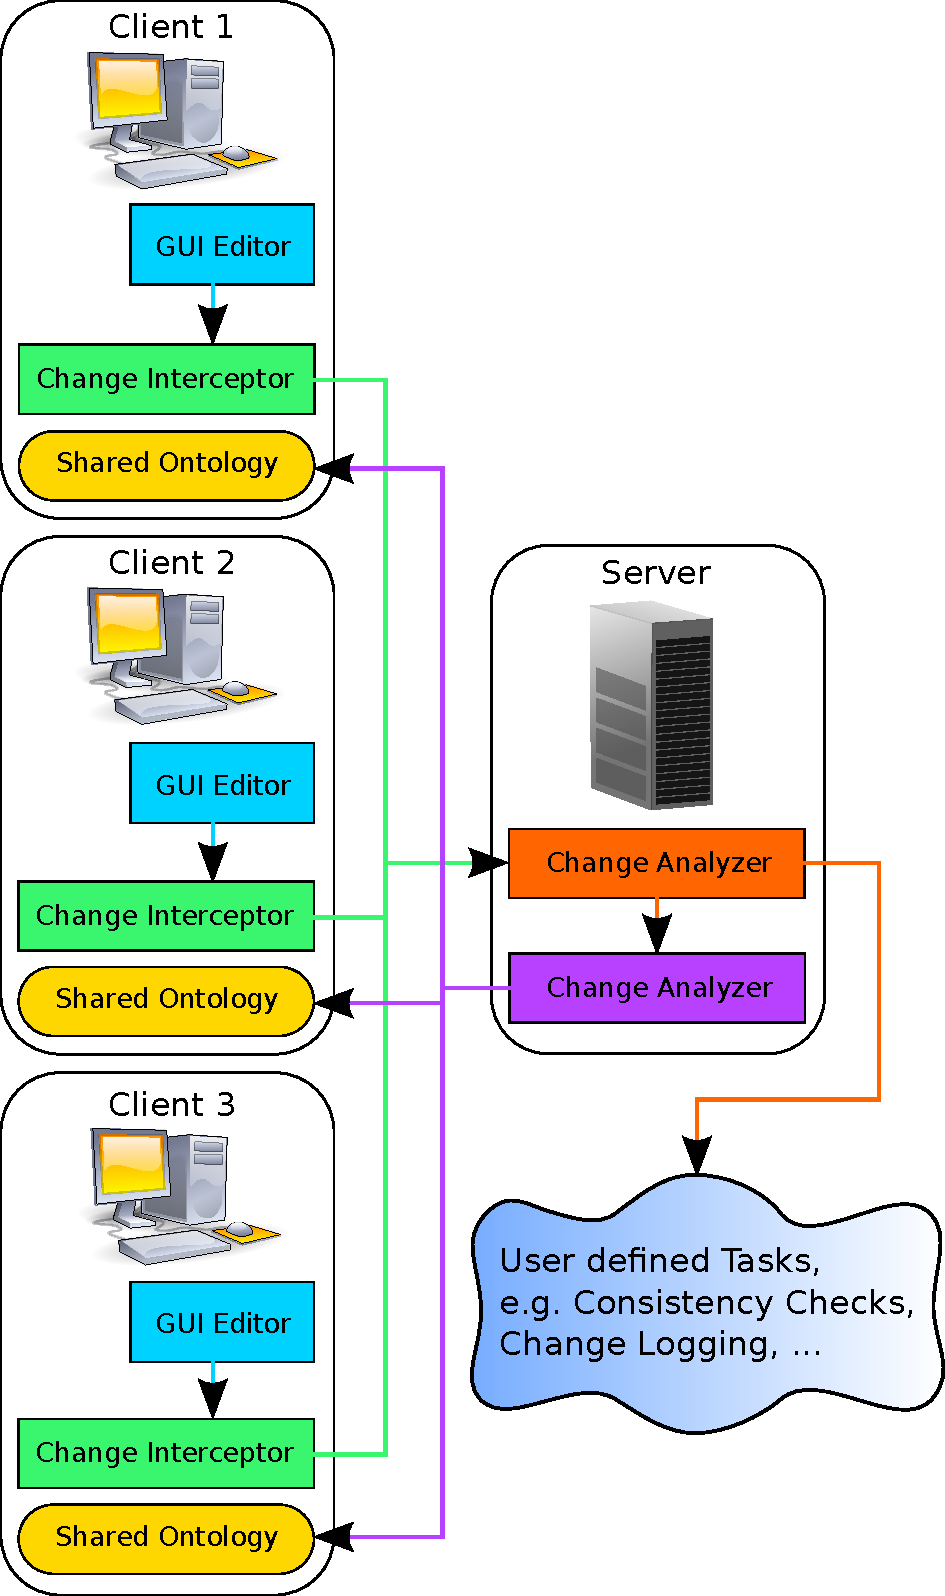
\includegraphics{BilderFrameworkArch/scenario0.pdf}
                                                }
                                        }
                                }
                                \label{img_scenario0}
                        }
                        \subfloat[Usage scenario 2]{
                                \rotatebox{0}{
                                        \resizebox{!}{0.6\textwidth}{
                                                \fbox{
                                                        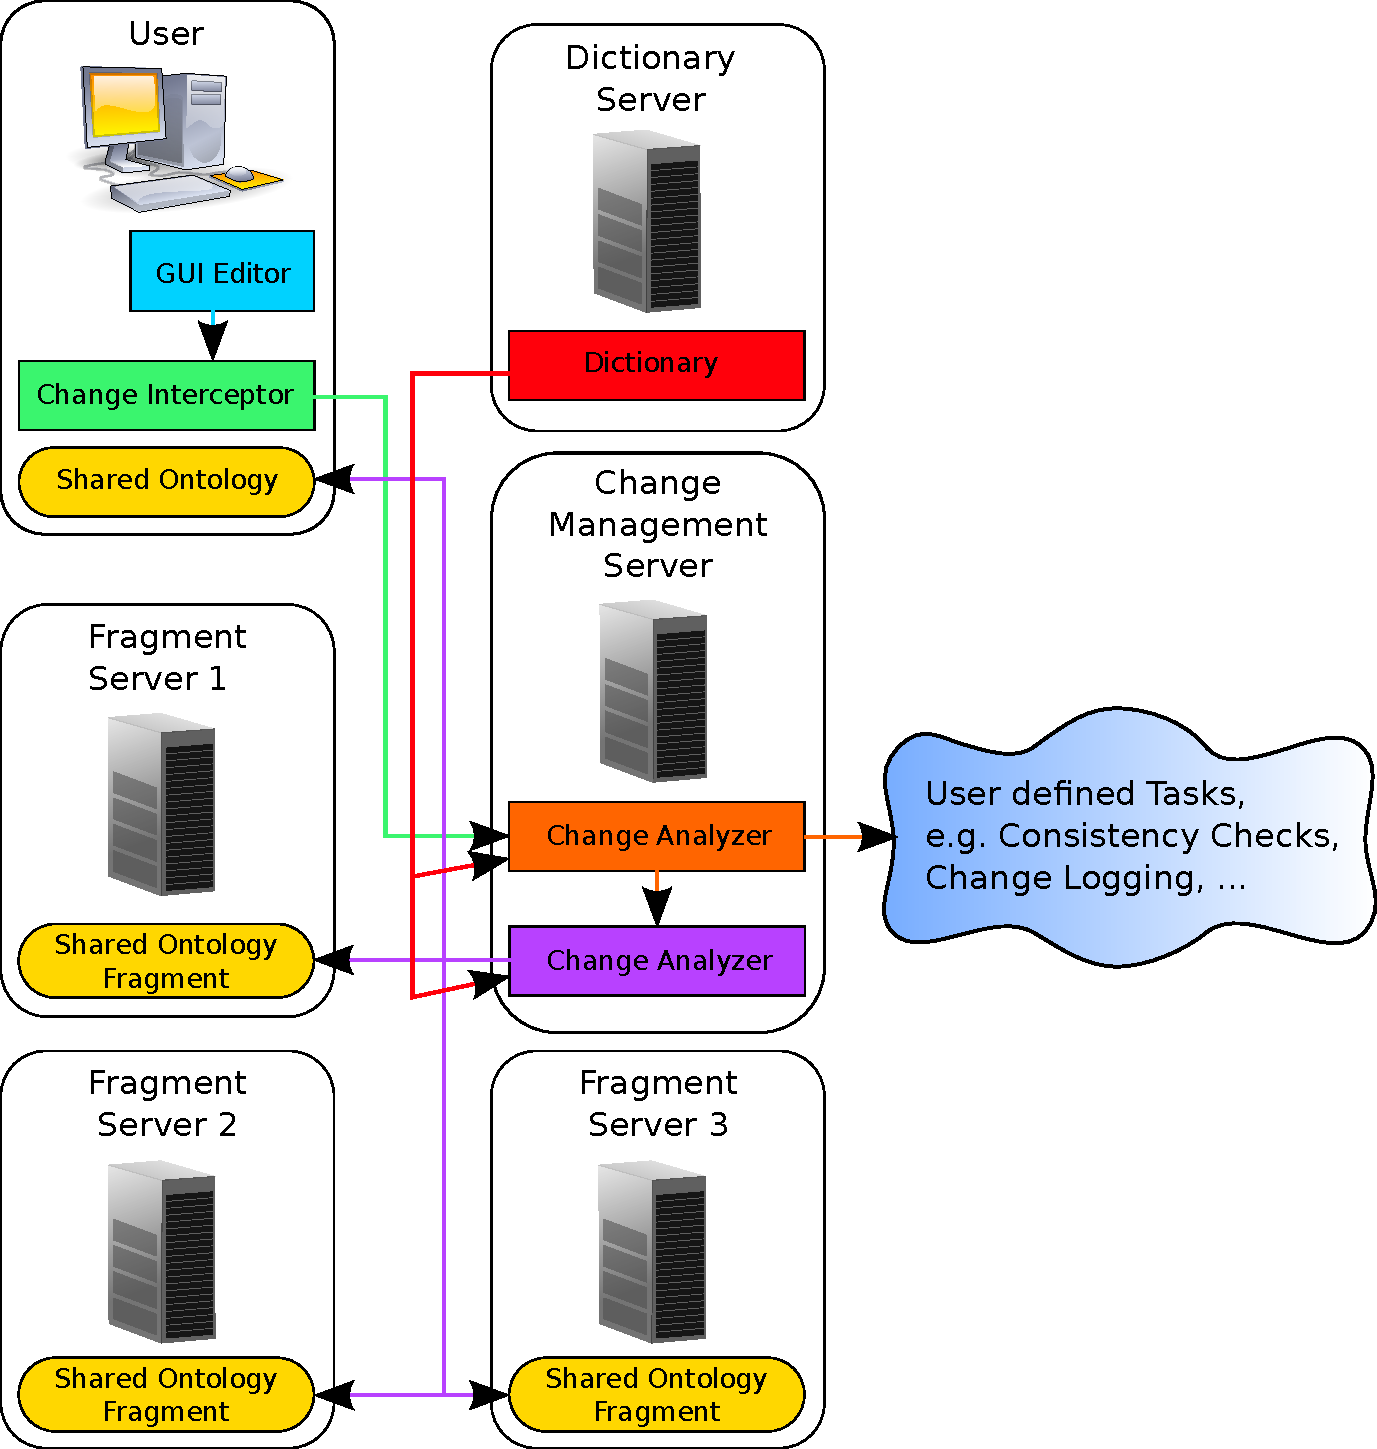
\includegraphics{BilderFrameworkArch/scenario1.pdf}
                                                }
                                        }
                                }
                                \label{img_scenario1}
                        }
        \label{fig_sharedontowizard}
\end{figure}
%\begin{figure}[h]
%       \caption{Usage scenario 1}
%       \begin{center}
%               \rotatebox{-90}{
%                       \resizebox{!}{0.45\textwidth}{
%                               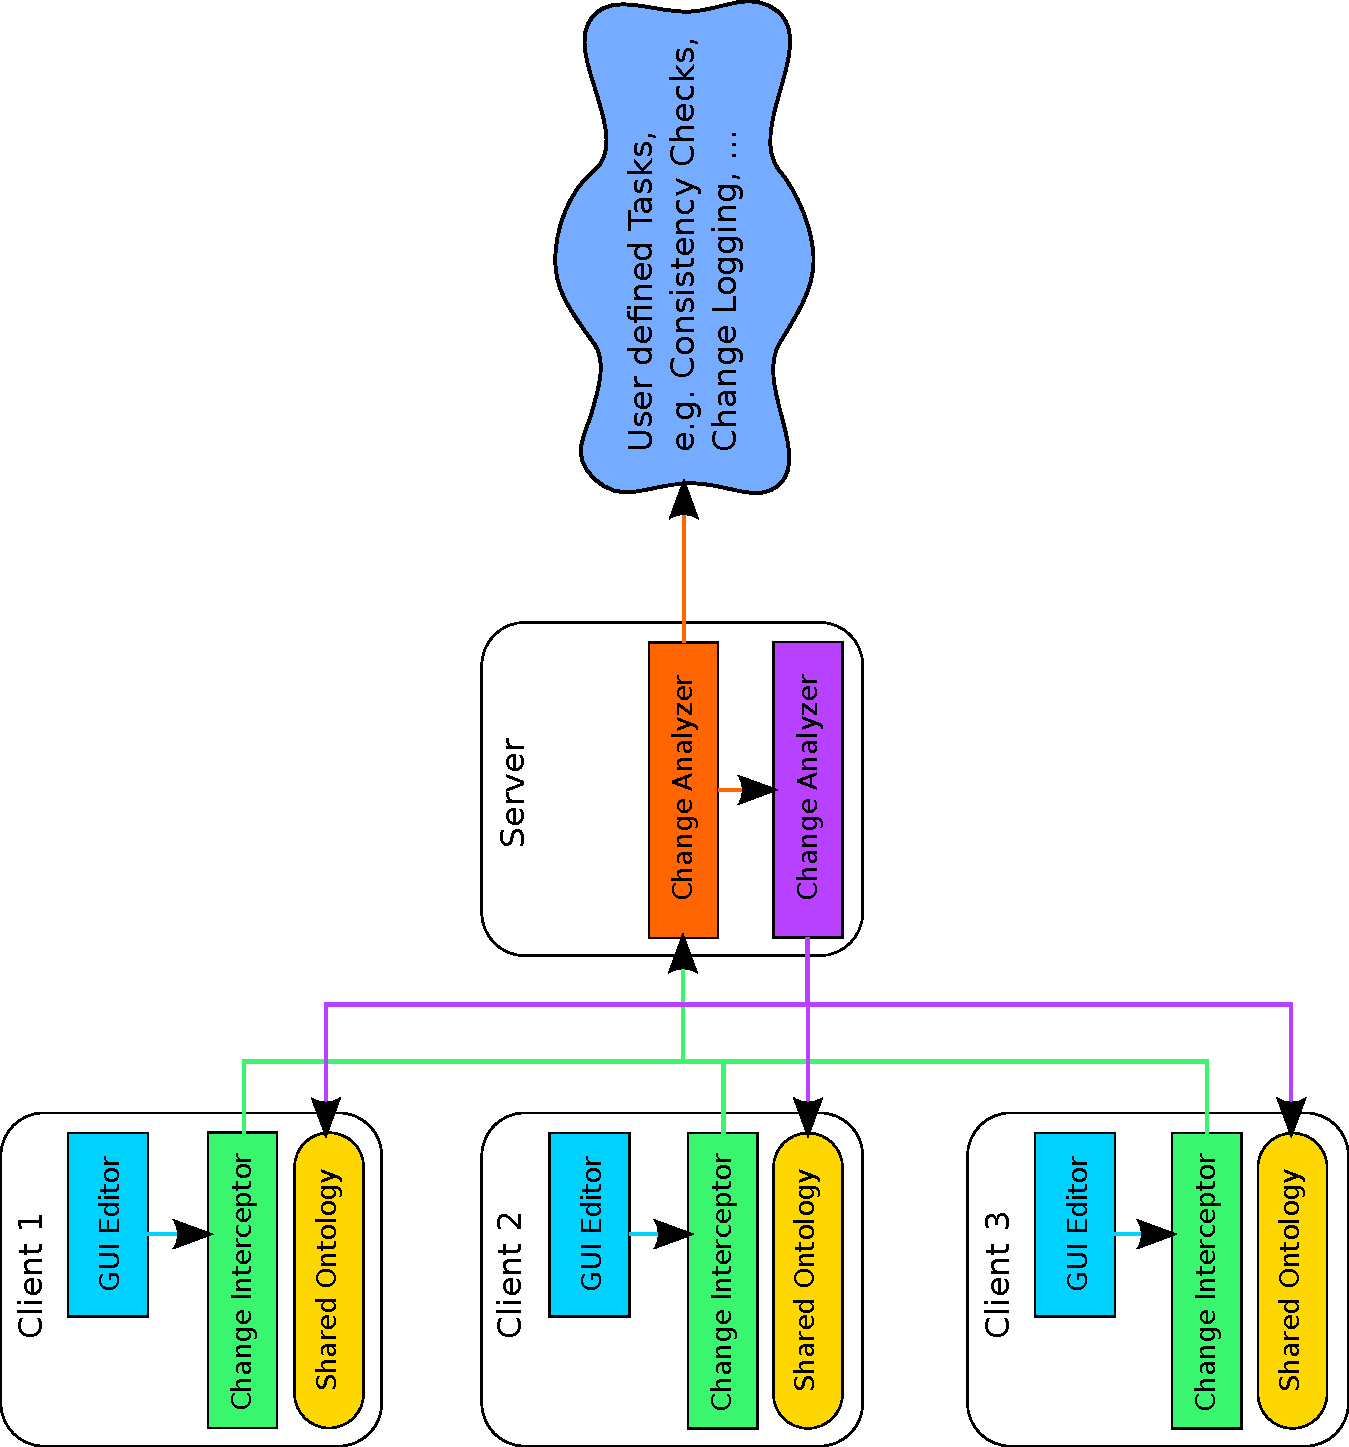
\includegraphics[width=10cm]{BilderFrameworkArch/component_overview0.pdf}
%                       }
%               }
%       \end{center}
%       \label{img_changemanagement}
%\end{figure}
%\begin{figure}[h]
%       \caption{Usage scenario 2}
%       \begin{center}
%               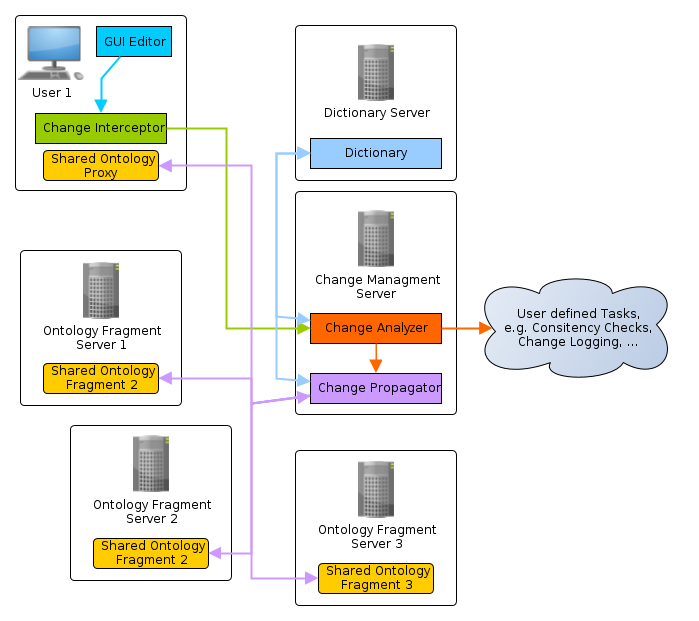
\includegraphics[width=10cm]{BilderFrameworkArch/component_overview2.png}
%       \end{center}
%       \label{img_changemanagement2}
%\end{figure}

\subsection{Shared Ontology}
\label{sharedOntology}
The key concept of the framework is the concept of a \emph{shared ontology}.
A shared ontology is an ontology which can be accessed and modified by
multiple clients. Working on a shared ontology is done synchronously which
means that changes are visible to all clients immediately after they have been made.
The defintion of a \emph{shared ontology} is based on the definition
in \cite{diaz2006}.

\begin{definition}[Shared Ontology] If an ontology is developed
through by publishing ontological contribution in contrast to developing
it through externalization we call it a \emph{Shared Ontology}.
\end{definition}

A shared ontology may be fragmented in smaller pieces which together
form the whole ontology. So a fragment is a subset of statements of the
ontology and is therefore an ontology itself.
Fragments can either be modular or non-modular.
Using modular fragments exposes several advantages which has been described
before in section \ref{modularization}.

\begin{definition}[Shared Ontology Fragment]
\label{sharedOntologyFragment}
For a Shared Ontology $o$ a set of axioms $\varphi$ is called a \emph{Shared Ontology Fragment}
of $o$ when $\varphi\subseteq o$.
\end{definition}

\subsection{Dictionary}
\label{dictionary}
The global dictionary contains meta information about fragments.
It covers fragment identifiers as well as fragment ontology signatures
and the \emph{identifier function} to look up a fragment by signature
and vice versa and is part of a distributed ontology system as proposed
in \cite{chen09}.
\begin{definition}[Identifier Function]
For a set $\mathcal{I}$ of ontology identifiers
and a set $\mathcal{F}$ of Shared Ontology Fragments
a bijective function $\phi$ : $\mathcal{I} \to \mathcal{F}$ that unambiguously assigns an identifier to every fragment is called an \emph{identifier function}.

\end{definition}
\begin{definition}[FragmentID]
For a set $\mathcal{I}$ of ontology identifiers,  a set $\mathcal{F}$ of Shared Ontology Fragments and a fragment $\varphi \in \mathcal{F}$, an identifier $\iota$ is called a \emph{FragmentID} of $\varphi$ if an identifier function $\phi$ exists such that $\exists \iota \in \mathcal{I} : \phi(\iota) = \varphi$. 
\end{definition}
Each Shared Ontology Fragment has a unique ID.
\begin{definition}[Dictionary]

For a set of FragmentIDs $\mathcal{I}_\varphi$, a set of Shared Ontology Fragments $\mathcal{F}$ and signature $\Sigma = \{{\sigma(\varphi)}\mid\varphi\in{\cal F}\}
$,
and $\phi$ an identifier function from ${\cal I}_\varphi$ to $\cal F$,
a triplet $\mathcal{D} = \{\mathcal{I}_\varphi, \Sigma, \phi \}$ is called
\emph{Dictionary}.

%\begin{enumerate}
%   \item $\Upsilon = \{ \iota set of fragment IDs
%   \item A set of ontology signatures $\Sigma = \bigcup_{i=1...n}{\sigma_i}$
%   \item Two functions $\phi$
%      $\texttt{getSignature} : \texttt{FragmentID} \to \texttt{Signature}$\\
%      $\texttt{getFragment} : \texttt{Signature} \to \texttt{FragmentID}$
%\end{enumerate}
\end{definition}
This offers the possibility to look up which fragment holds required information
when performing a query against a distributed ontology which is also
the primary purpose of the dictionary.
The dictionary can be further extended to contain other information about fragments
if needed such as the fragment size or structural properties.

%\begin{enumerate}
%\item Each concept name $\DLConVar{A}\in N_C$ is an \ALC-concept description.
%\item The most general concept $\top$ and the unsatisfiable concept $\bot$ are \ALC-concept descriptions.
%\item If \DLConVar C, \DLConVar D are \ALC-concept descriptions, and $\DLRolVar{R}\in N_R$, then  the concept conjuntion $\DLConVar C \DLand \DLConVar D$, the concept disjunction $\DLConVar C \DLor \DLConVar D$ and the concpet negation $\neg\DLConVar{C}$ are also \ALC-concept descriptions.
%\end{enumerate}


\newpage


\subsection{Distributed Ontology System}
\index{DOS}
We adapt the concept of a  \emph{Distributed Ontology System} (DOS)
proposed by \cite{chen09}. A DOS consists of a large shared ontology
a set of ontology fragments the ontology is composed of and a dictionary
to look up fragments.

\begin{definition}[Distributed Ontology System] For a large shared ontology
$o$, a set of ontology fragments $\mathcal{F}$ which $o$ is composed of
and a dictionary $\mathcal{D}$, a triplet $\{o,\mathcal{F},\mathcal{D}\}$
is called \emph{Distributed Ontology System}.
\end{definition}

\subsection{Change Management}
\label{changemanagement}
This sub section presents components related to change management in
the Replica Framework.

When it comes to the distribution of a shared ontology the Replica Framework has
to provide the means for managing changes. Each node provides special
components which allocate all necessary functionalities for \emph{change management}
from intercepting changes to analyzing and propagating them which are
also the three stages in order in which change is processed.

\subsubsection{Change Model}
The framework does not force the user into using a certain change distribution
model. By exhausting the full functionality of the change management
the Replica Framework offers the flexibility to implement change management
according to user's demands.

The forms of ontology modifications are diverse. Users can add or
remove axioms to shared ontologies or certain fragments, add annotations
or change the ontology ID. Moreover users may want to apply a set of these
modifications. Keeping track of modifications is essential in many applications
for example in versioning systems.

\begin{definition}[Change]
For the set $\Delta$ of ontology modifications, user ID $\upsilon$,
time~stamp~$\tau$, comment $\omega$, the 4-tuple 
$\mathcal{\nu} = \{\Delta, \upsilon, \tau, \omega \}$ is called \emph{change}.
\end{definition}
The Replica Framework uses a special container called \emph{change} to
carry a set of modifications, a user ID, a timestamp and a comment which
is meant to report the cause of the change.
%\begin{tabular}{ l l }
%Change: applyChange(c)

\begin{definition}[Criterion] 
A \emph{criterion} is a function $Change \to Boolean$ that
 \emph{matches} a change.

\end{definition}
Note that a \emph{Change} can contain a set of modifications.

\begin{definition}[Change Filter]
For $n \in \mathbb{N}$, Criteria $\gamma_i$, 
$\Theta = \bigcup_{i=0..n} \gamma_i$ is called \emph{Change Filter}.
\end{definition}
A \emph{Change Filter} is meant to be used at the first step of the change
processing but also in any other component where changes are handled.

\subsubsection{Change Processing}
Change processing in the Replica Framework follows a scheme which can be
modified if needed. Developers can implement custom modifications and
other tasks in any component. Figure \ref{img_changeprocessing} presents
the change processing work flow.
\begin{figure}[h]
        \caption{Change processing work flow}
        \begin{center}
                 \rotatebox{-90}{
                        \resizebox{!}{10cm}{
                                
\includegraphics[width=10cm]{BilderFrameworkArch/change_processing_flow.pdf}
                        }
                }
        \end{center}
        \label{img_changeprocessing}
\end{figure}\\
Whenever a change is applied this procedure is triggered. Next change
processing is described in algorithm \ref{alg_applychange} which
describes the change processing in detail.
\begin{algorithm}[h]                      % enter the algorithm environment
\caption{\textsc{ApplyChange($\mathcal{\nu}$)}}          % give the algorithm a caption
\label{alg_applychange}                           % and a label for \ref{} commands later in the document
\begin{algorithmic}[h]                    % enter the algorithmic environment
\REQUIRE Shared Ontology $o$, Change Filter $\Theta$
\IF{\NOT \textsc{Filter($\mathcal{\nu}, \Theta$)}}
        \STATE{$\alpha \leftarrow \textsc{Analyse($\mathcal{\nu}$)}$
        \STATE \textsc{Trigger($\alpha$)}
        \STATE \textsc{Propagate($\alpha,\mathcal{\nu}$)}}
        \RETURN applied changes on $o$
\ELSE
        \STATE // ignore change
\ENDIF
\end{algorithmic}
\end{algorithm}\\
The other procedures used in algorithm \ref{alg_applychange} are:
\begin{algorithm}[h]                      % enter the algorithm environment
\caption{\textsc{Filter($\mathcal{\nu}, \Theta$)}}          % give the algorithm a caption
\label{alg_filter}                           % and a label for \ref{} commands later in the document
\begin{algorithmic}[h]                    % enter the algorithmic environment
\REQUIRE Criteria $\chi_i \in \Theta$\hspace{0,5cm} $i = 1,2,...,n$\hspace{0,5cm} $i,n \in \mathbb{N}$
\FOR{$i = 1\text{ to }n$}
        \IF{$\chi_i(\mathcal{\nu})$}
                \RETURN \TRUE
        \ENDIF
\ENDFOR
\RETURN \FALSE
\end{algorithmic}
\end{algorithm}
\begin{itemize}
        \item[\textsc{Analyse}]  is a developer-defined analysis procedure that examines a change
        and returns an analysis as a result. The Replica Framework poses no
        restrictions on the subject and content of this analysis.
        \item[\textsc{Trigger}] is also a developer-defined algorithm that depends on the
        analysis. This algorithm may for example be a consistency check of
        the ontology or protocolling a change.
        \item[\textsc{Propagate}] is the function that sends a change to other peers.
        To which peers the change is sent depends on the developers demands.
        The change can also be modified at this stage.
\end{itemize}

%\begin{algorithm}[h]                      % enter the algorithm environment
%\caption{\textsc{Analyse($\mathcal{\nu}$)}}          % give the algorithm a caption
%\label{alg_analyses}                           % and a label for \ref{} commands later in the document
%\begin{algorithmic}[h]                    % enter the algorithmic environment
%\REQUIRE Shared Ontology $\mathcal{O}$
%\STATE $\alpha \leftarrow$ Create change analysis
%\STATE \textsc{Trigger($\alpha$)}
%\RETURN $\alpha$
%\end{algorithmic}
%\end{algorithm}

\subsubsection{Change Interceptor}
The \emph{Change Interceptor} is responsible for intercepting and if required
filtering changes on the shared ontology. Filters are be based on the node
a change originates from and also the kind of change.

This component is local on a node. After a change has been intercepted
it is either modified and forwarded to the change analyzer or filtered.

\subsubsection{Change Analyzer}
The \emph{Change Analyzer} component is used to inspect the change type
and possibly trigger user defined tasks connected to certain outcomes of the
analysis. A user defined task may for example be a consistency check or some
other kind of check for constraints. This offers workflow support.

Changes can also be filtered at this component. The main difference to the
change interceptor is that the change analyzer can either be distributed thus 
local on any node or at certain user specified hosts. This allows centralizing
change analysis and easy change tracking for building change histories.

\subsubsection{Change Propagator}
\label{changepropagator}
At last the \emph{Change Propagator} component is required to send the
shared ontology change to all or some other nodes. The Change Propagator
should know the analysis of the change produced by the Change Analyzer.
In addition to that a change propagation strategy should be configurable. The
strategy determines which changes will be sent to specified nodes.
It is therefore a very important aspect of the framework. The strategy can either
be configured to propagate changes to all or just some nodes.
The target node(s) of a certain change can also depend on the kind of change
which is about to be propagated or other developer defined information.


\subsection{Communication Node}
The framework relies on a client and server communication model.
Clients connect to a server and can then retrieve shared ontologies managed
by the server they are connected to as well as changes and communication
data from other clients. As centralization is not always desired the
framework also allows for building decentralized network structures
by employing the concept of a \emph{communication node}.
A communication node is a peer that provides client as well as server functionality.

The concept of a communication node is similar but not equal to the
peer concept of a peer-to-peer network. Table \ref{p2pRepComparison}
offers a comparison between the two ideas which is based on the definition
of a peer-to-peer network by \cite{schollmeier01}.
The major difference between both network models is that in opposite to
a self-organizing peer-to-peer network communication node management has
to be configured manually.

\begin{table}[h]
        \centering
        \caption{Comparison of peer-to-peer and Replica Framework peer concepts}
        \label{p2pRepComparison}
        \begin{tabular}{ | p{0.60\textwidth} | c | c | }
                \hline
                \textbf{Characteristic} & \textbf{Peer-to-Peer} & \textbf{Replica Framework} \\ \hline
                Heterogenity of network connection speed, performance, reliability & yes &  yes \\ \hline
                Peers provide services and resources and request services of other peers & yes & yes \\ \hline
                Services and resources can be shared across all peers & yes & yes \\ \hline
                Peers make up an overlay network & yes & yes \\ \hline
                Peers are autonomous & yes & yes \\ \hline
                The network is self-organizing & yes & no \\ \hline
        \end{tabular}
\end{table}

\section{Behavioral Aspects}
This section outlines an important behavioral aspect of the Replica Framework
architecture. \emph{Change Management} is described, the
concept and a simple standard management strategy that a
framework implementation should provide as a starting point.

\subsection{Change Management}
\label{changemanagement_behave}
In some usage scenarios not all users may be allowed to submit changes or
enforcing restrictions is necessary. Furthermore changes may need to
be modified before applying them to the shared ontology or it may be necessary
to trigger an event when a certain type of change is submitted.
Performing a consistency check before applying a change is an example for
such a situation where change management is required.

To offer a maximum of flexibility a change can be filtered and modified
at any stage in change processing: (1) interception (2) analysis (3) tasks
and (4) propagation.

\subsubsection{Change distribution}
A fundamental aspect of change management is the distribution of changes.
The easiest change distribution model is plain synchronous unmodified change
distribution. All changes made on a node are instantly transmitted without
modification. By defining a change propagation strategy for the
\emph{change propagator} component presented in section \ref{changepropagator}.


\section{System Configuration}
Each Replica Framework component may require a configuration supplied by the user.
Whenever possible reasonable defaults are used which can then be overridden by
supplied configuration values. To simplify the configuration process a bundle
of the individual component configurations can be created and be read at
a central place. The Replica Framework takes care of distributing and applying
the configurations to corresponding components.

